% !TeX spellcheck = en_US
\addsection{Combat}{\skills/attack.png}

\begin{multicols}{2}

\hypertarget{Combat}{Combat}\index{Combat} with \textbf{Neutral Units} starts when a Hero moves to an unvisited Field with a roman numeral, signifying the \hyperlink{Difficulty}{type and number} of Neutral Units guarding that Field.

Combat with \textbf{another player} can start in two ways:
\begin{itemize}
  \item You move into any Field containing one of their Heroes.
  \item You move into a Town or Settlement owned by them.
\end{itemize}
Players are able to start multiple Combats during their Turn.

\subsection*{\hypertarget{Combatsetup}{Combat Setup}}

% TODO info about battlefield expansion
Combat is resolved on the 4 x 5 Combat board, which consists of two Backlines and two Frontlines on opposite ends, and a middle row.
Follow these steps when Combat begins against \textbf{Neutral Units}:

\begin{itemize}
  \item Choose one of the Combat Board's sides as your own.
    Place up to 5 of your Unit cards freely onto the Back and Frontlines of that side.
  \item Check the \hyperlink{Difficulty}{\textbf{Difficulty Table}} and draw the corresponding number of Neutral Unit cards from their Decks.
  \item The Neutral Units are placed differently depending on the Game Mode:
  \item In \textbf{Clash} or \textbf{Alliance} Scenarios, the enemy player sitting to your right controls the Neutral Units and decides their placement.
    \includesvg[height=10px]{\svgs/unit_ranged.svg} Units must be placed in the Backline if possible.
  \item In \textbf{Campaign} or \textbf{Cooperative} scenarios, Neutral Units are placed from left to right from the player's perspective.
First, place any \includesvg[height=10px]{\svgs/unit_ranged.svg} Units in the Backline\index{Units Placement}.
Then, place any \includesvg[height=10px]{\svgs/unit_ground.svg} or \includesvg[height=10px]{\svgs/unit_flying.svg} Units in the Frontline.
If there's not enough room to place a Unit in its correct line, place them in the other one.
Units must be placed in \textbf{descending} Initiative\index{Initiative} order.
If there's a tie, place higher tier Units first.
If there's still a tie, the players decide the order.
\end{itemize}
Unit setup when fighting \textbf{other players}:
\begin{itemize}[wide]
  \item The attacking player places up to 5 Units on their chosen side of the Combat Board, followed by the defender.
  \item If the Combat takes place in a Town with a Citadel, the defender adds the \hyperlink{Walls}{Wall, Gate and Arrow Tower} cards after placing their Units.
\end{itemize}
\vfill
\begin{center}
  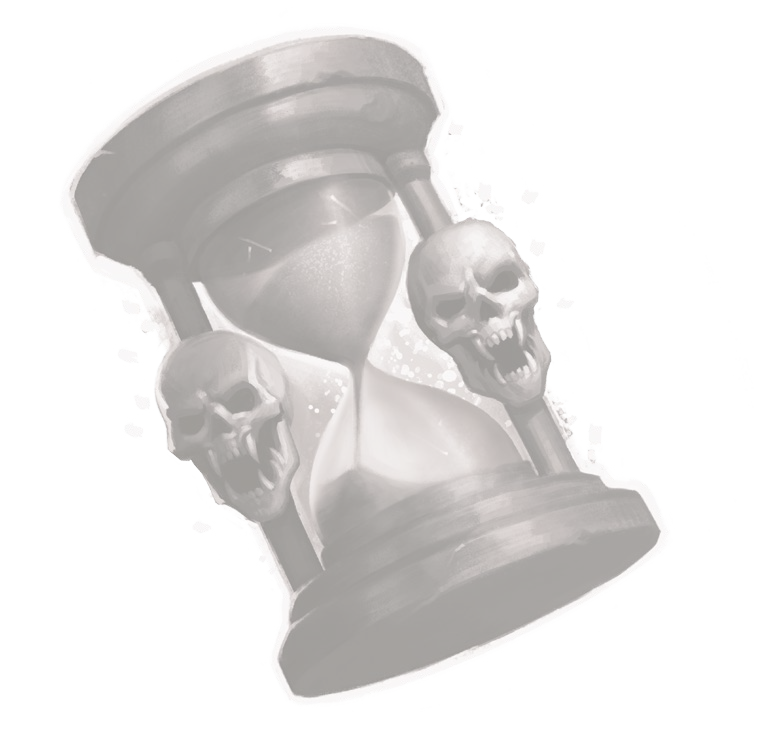
\includegraphics[width=0.55\linewidth]{\art/aging.png}
\end{center}
\vfill
\note{11}{
    If your Town or Settlement is attacked by an enemy Hero and your Hero is not on that Field, you may immediately \textbf{pay 8} \includesvg[height=10px]{\svgs/gold.svg} to fight a defending Combat \textbf{using only your Units}.
    You cannot use your Deck during that Combat as your Main Hero is not present.
    Paying this Gold represents the cost of transporting the army there.
}

\subsection*{\hypertarget{Combatterminology}{Combat Terminology}}
The following terms are used to describe effects and elements during Combat:\par
\textbf{Attacking Player} – The player who started the Combat.\par
\textbf{Defending Player} – The player whom Combat was started against.\par
\textbf{Activation} – A Unit Activates when it is next in the Initiative order.\par
\textbf{Adjacent Unit} – A Unit is directly adjacent to another if it is one space away in a cardinal direction (nondiagonal).\par
\textbf{Combat Round} – A full cycle of all Units of each player being Activated.\par
\textbf{Combat Obstacles}\index{Combat Obstacles}\index{Obstacles, Combat} – Every card on the Combat Board is a Combat Obstacle.
They block the movement of all non-flying Units.\par
\textbf{Attack Die}\index{Attack Die} – A red Die whose results range from -1 to +1.
Roll the Die \textbf{whenever a Unit attacks} and
add the result to the Unit's Attack value.\par
\textbf{\hypertarget{Retaliate}{Retaliation Attack}} – If a Unit survives an attack by an adjacent Unit, it performs an attack back at that Unit.
Each Unit can perform \textbf{only 1} Retaliation Attack\index{Retaliation Attack} per Combat Round.
Retaliation Attacks function identically to normal attacks, but they cannot cause another Retaliation Attack.
Mark Units which have performed a Retaliation Attack this Round with a black cube.\par
\textbf{Paralysis}\index{Paralysis} \includesvg[height=10px]{\svgs/paralysis.svg} – Some effects place a Paralysis Token on Units.
That Unit \textbf{must skip its next Activation}. Remove the Token instead of activating it.
If the Unit \textbf{attacked or takes any damage} before that time, \textbf{remove the Token}.
The Token does not prevent Units from performing Retaliation Attacks.\par
\textbf{\hypertarget{Defend}{Defend}} \includesvg[height=10px]{\svgs/defense.svg} – Units may choose to gain a Defense Token instead of attacking.
When a Unit with a Defense Token is attacked, make another roll with the attack Die after the initial attack roll.
If you roll a "+1", the defending Unit gains an extra 1 Defense for this attack.
If a Unit has a Defense Token at the start of its activation, discard it.
The Unit cannot take another Defense Action during that activation.

\subsection*{\hypertarget{CombatCards}{Using Cards During Combat}}
You may only use \textbf{one Spell per Combat Round}.
Ongoing \includesvg[height=10px]{\svgs/ongoing.svg} and \includesvg[height=10px]{\svgs/activation.svg} Activate effects can be used only \textbf{when Activating one of your Units and before it attacks}.
Ongoing effects\index{Ongoing Effects} last until end of Combat or if the effect on the card is used up.\par
Instant \includesvg[height=10px]{\svgs/instant.svg} Cards may be played \textbf{at any time} except between rolling the Combat Die and resolving damage unless otherwise stated.
Instant Cards which increase a Unit's \includesvg[height=10px]{\svgs/attack.svg} or \includesvg[height=10px]{\svgs/defense.svg}, such as the Attack and Defense Statistic cards, \textbf{must} be played after an attack has been announced and persist only for the duration of that attack.
\subsection*{\hypertarget{Timelimit}{Combat Time Limits}}\index{Time Limit}
Combats against Neutral Units have a time limit of \textbf{one Combat Round}.
If you cannot win the Combat before the end of the current Combat Round, you must either \hyperlink{Endcombat}{Retreat}\index{Retreat} or spend 1 MP from the Hero that started the Combat in order to play another Round.\par

\bigskip

\note{5}{Combats against Azure \includesvg[height=10px]{\svgs/azure-note.svg} Units, other players, or \hyperlink{AIrules}{AI Heroes} have no time limit.}

\vfill

\begin{center}
  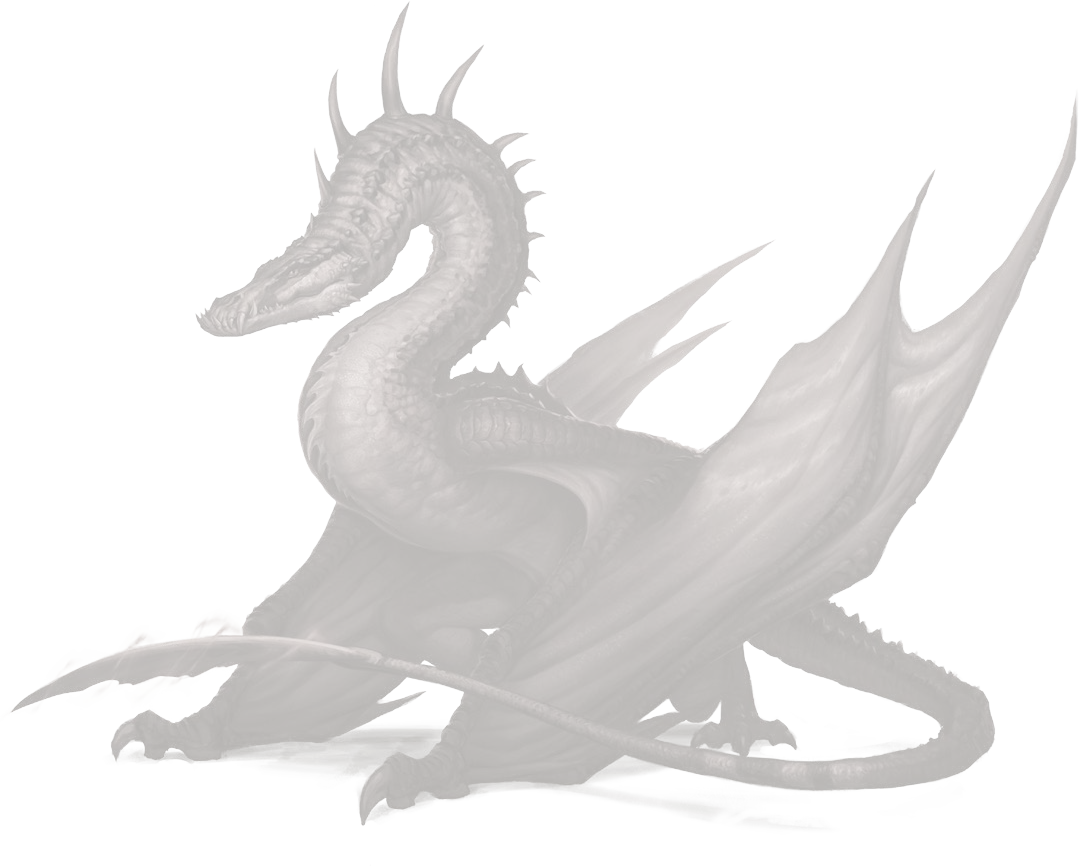
\includegraphics[width=0.7\linewidth]{\art/wyvern.png}
\end{center}

\filbreak

\subsection*{\hypertarget{Walls}{Defending a Town With\\a Citadel\raggedright}}\index{Defending Town}

When a Town with a Citadel is attacked, the defender adds the 3 Wall and 1 Gate Obstacles in any order to the Middle Row of the Combat Board after placing their Units.
The Gate Card is \textbf{not an Obstacle to the defending player}.
The Wall and Gate\index{Walls and Gate} cards can be destroyed by any adjacent \includesvg[height=10px]{\svgs/unit_ground.svg} or \includesvg[height=10px]{\svgs/unit_flying.svg} Unit's attack.
\par
Defending Units standing on their own side and \textbf{in the same column} as a Wall or a Gate gain protection from \includesvg[height=10px]{\svgs/unit_ranged.svg} attacks.
If they are targeted by a \includesvg[height=10px]{\svgs/unit_ranged.svg} attack performed from the opponent's side of the Combat Board, \textbf{reduce the attack's damage by 1}.

\begin{center}
  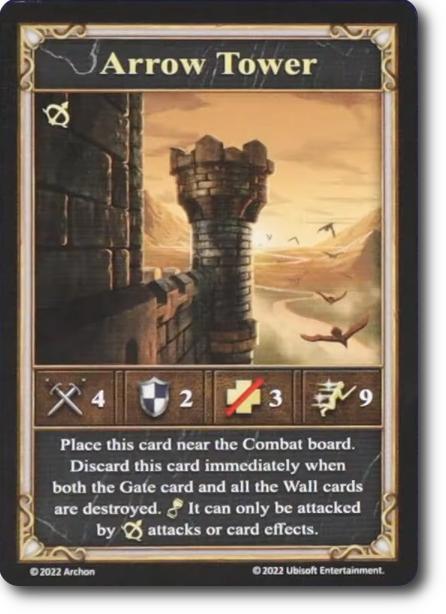
\includegraphics[width=0.6\linewidth]{\cards/arrow_tower.png}
\end{center}
The defender also gains the Arrow Tower\index{Arrow Tower} Unit Card which is placed next to the Combat Board.

\end{multicols}

\vspace*{\fill}
\begin{figure*}[h]
  \mbox{}%
  \hfill%
  \begin{minipage}[t]{0.415\textwidth}
    \centering
    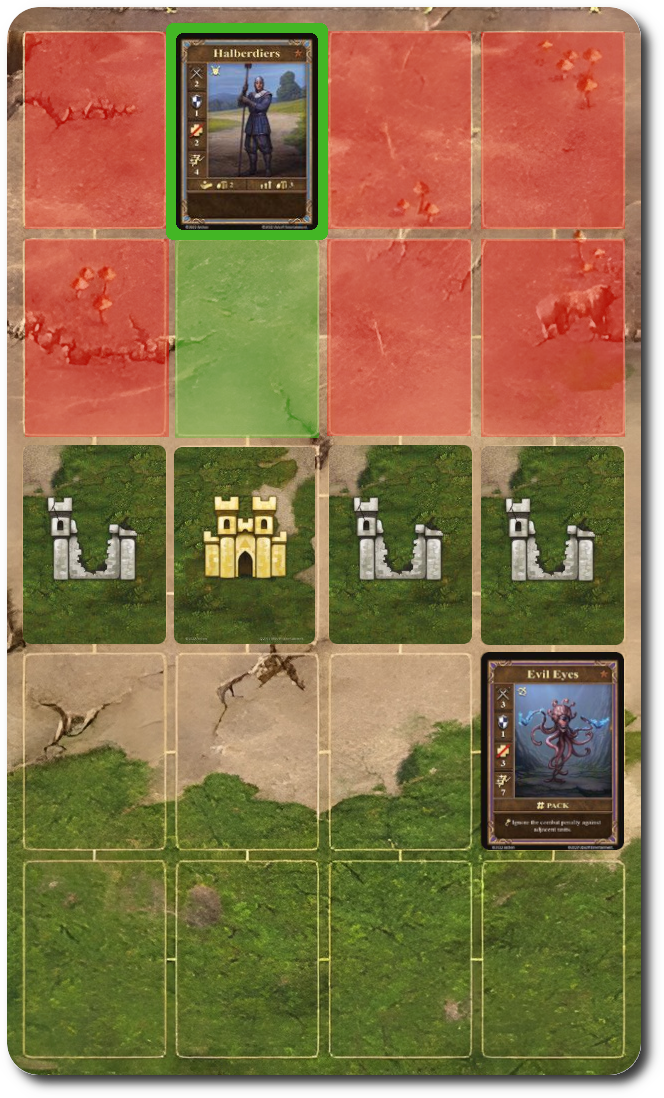
\includegraphics[width=\linewidth]{\examples/ranged_protected.png}
  \caption[halberdiers protected]{\textit{When the Halberdiers are behind a non-destroyed Gate, they \textbf{are protected} when attacked from behind the Wall line.
    The \includesvg[height=10px]{\svgs/unit_ranged.svg} attack damage of Evil Eyes is \textbf{reduced by 1}.}}
  \end{minipage}
  \hfill%
  \begin{minipage}[t]{0.415\textwidth}
    \centering
    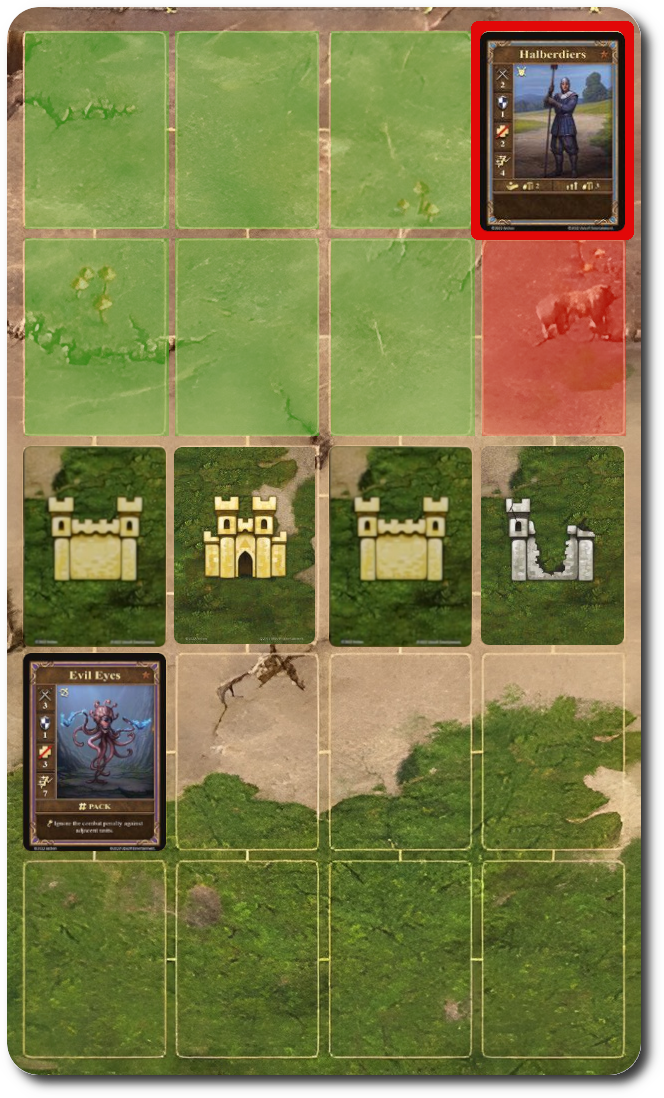
\includegraphics[width=\linewidth]{\examples/ranged_unprotected.png}
    \caption[halberdiers unprotected]{\textit{Because the Halberdiers are not behind a non-destroyed Wall, \textbf{protection doesn't work}.
      Evil Eyes attack \textbf{without penalty}.}}
  \end{minipage}
  \hfill%
  \mbox{}%
\end{figure*}

\begin{multicols}{2}

\subsection*{Combat Round Structure}
Combat is divided into Rounds, during which all of the Units participating in that Combat \textbf{Activate once} in Initiative order.
After each Unit has Activated, a new Combat Round begins.
Combat lasts until all Units on one side are eliminated, a player has to \textbf{Retreat} when fighting Neutral Units, or a player \textbf{Surrenders} to another player.

Structure of a Combat Round:
\begin{itemize}
  \item Players Activate their Units in descending order of Unit \hyperlink{Initiative}{Initiative}. \textbf{If there's a tie}, alternate between attackers and defenders starting with an attacker.
  \item When a Unit Activates, place a Faction Cube on it to indicate it has been Activated this Combat Round.
  \item Activated Units may move and attack according to their \hyperlink{Unittype}{type}. Neutral Units controlled by an opposing player must always attack if possible.
  \item Instead of attacking, a Unit may \hyperlink{Defend}{defend}.
  In Neutral Combat, the Neutral enemy Units cannot defend, even when controlled by another player.
  \item Before a Unit attacks, both players may \hyperlink{CombatCards}{play Cards}. Cards are resolved in the order in which players decide to play them.
  \item After a Unit's attack has been declared and all cards have been played, roll the Combat Die.
    Modify the attacking Unit's attack by the Die's result, then reduce it by the defending Unit's Defense, and finally deal the rest as \hyperlink{HP}{damage} to the defending Unit.
  \item If the defending Unit was adjacent to the attacker, it \hyperlink{Retaliate}{retaliates} if it hasn't done so this Round.
  \item Keep activating Units until they've all been Activated once.
After the last Unit's activation, the Combat Round ends.
\end{itemize}

\subsection*{\hypertarget{Endcombat}{End of Combat}}
Combat ends immediately if all units on one side are defeated.
The side with any surviving units is the winner.
In Combat against \textbf{Neutral Units}, if you \hyperlink{Timelimit}{run out of time} or your Units are defeated, you must \textbf{Retreat}; move any surviving Units back to your Unit Deck and move the Hero that started the Combat back to the Field they \textbf{last Visited}.
There are no other negative consequences to Retreating.\par
\note{9}{
  \textbf{Important exception}: If \textbf{all} of your Units from your \textbf{Unit Deck} were defeated during Neutral Combat, your Main Hero must be moved to a friendly Town or Settlement.
  Secondary Heroes are removed from the game until Recruited again.\par
}\par
If you defeat all Units during Combat against \textbf{another player's Main Hero}, the defeated player \textbf{loses Morale} and has to \textbf{pay the winner} 5 \includesvg[height=10px]{\svgs/gold.svg}.
Do not lose Morale or pay \includesvg[height=10px]{\svgs/gold.svg} if a \textbf{Secondary Hero} is defeated.
\textbf{In both cases}, the defeated player also \textbf{gives the winner} one of their \hyperlink{End}{Faction Cubes}.
Defeated Main Heroes \textbf{have to move} to a friendly Town or Settlement, while Secondary Heroes are removed from the game until Recruited again.
Defeating a Main Hero may cause \hyperlink{End}{Player Elimination}.\par
You may \textbf{Surrender}\index{Surrender} to another player by paying them 10 \includesvg[height=10px]{\svgs/gold.svg} when activating a Unit.
Move your Main Hero or remove your Secondary Hero from the game as if you were defeated by losing your Units.
There are no other direct consequences to Surrendering; the winner does not gain a Faction Cube.\par
\note{4}{You cannot surrender when defending a Town.}\par
When a Secondary Hero is attacked, they may also choose to be \textbf{instantly defeated} instead of fighting a Combat in order to preserve their Units.
When this happens, the attacker still receives a Faction Cube from the defeated Hero.\par
When Combat ends, all damage is healed from all surviving Units.
Move any player owned Units back to their Unit Deck and discard any leftover enemy Neutral Units.
After winning Combat, Heroes \textbf{must} Visit the Field where the Combat took place.

\subsection*{\hypertarget{Combatexperience}{Combat Experience}}

Winning Combat with your Main Hero usually grants them Experience\index{Experience}.
If either the Difficulty of the Neutral Field or the Level of a defeated enemy Main Hero was \textbf{equal} to your Level, gain 1 \includesvg[height=10px]{\svgs/experience.svg}.
If they were \textbf{higher} than your Level, gain 2 \includesvg[height=10px]{\svgs/experience.svg}.
Winning a Neutral Combat against a Neutral Azure \includesvg[height=10px]{\svgs/azure.svg} Unit grants your Hero Level 7 \textbf{immediately}.
If you ever gain multiple Levels at the same time, resolve their effects in order.
Level ups must be resolved before Visiting the Field where the Combat happened.\par
Secondary Heroes cannot ever gain Experience.
You also do not gain Experience from \textbf{defeating} a Secondary Hero, or if an enemy Hero \textbf{Surrenders} to you.

\subsection*{\hypertarget{Quick}{Quick Combat}}\index{Quick Combat}
If your Hero's Level is higher than a Field's Difficulty when Combat against Neutral Units would begin, \textbf{no Combat} takes place.
The player is considered to have beaten the Neutral Units by default and gains no rewards from the Combat.

\subsection*{Campaign and Cooperative Combat}
During these game modes, all enemy Units activate according to the rules in \hyperlink{AIrules}{the next section}.

\end{multicols}

\vspace*{\fill}
\begin{scaledfigure}[blanker]
  \centering
  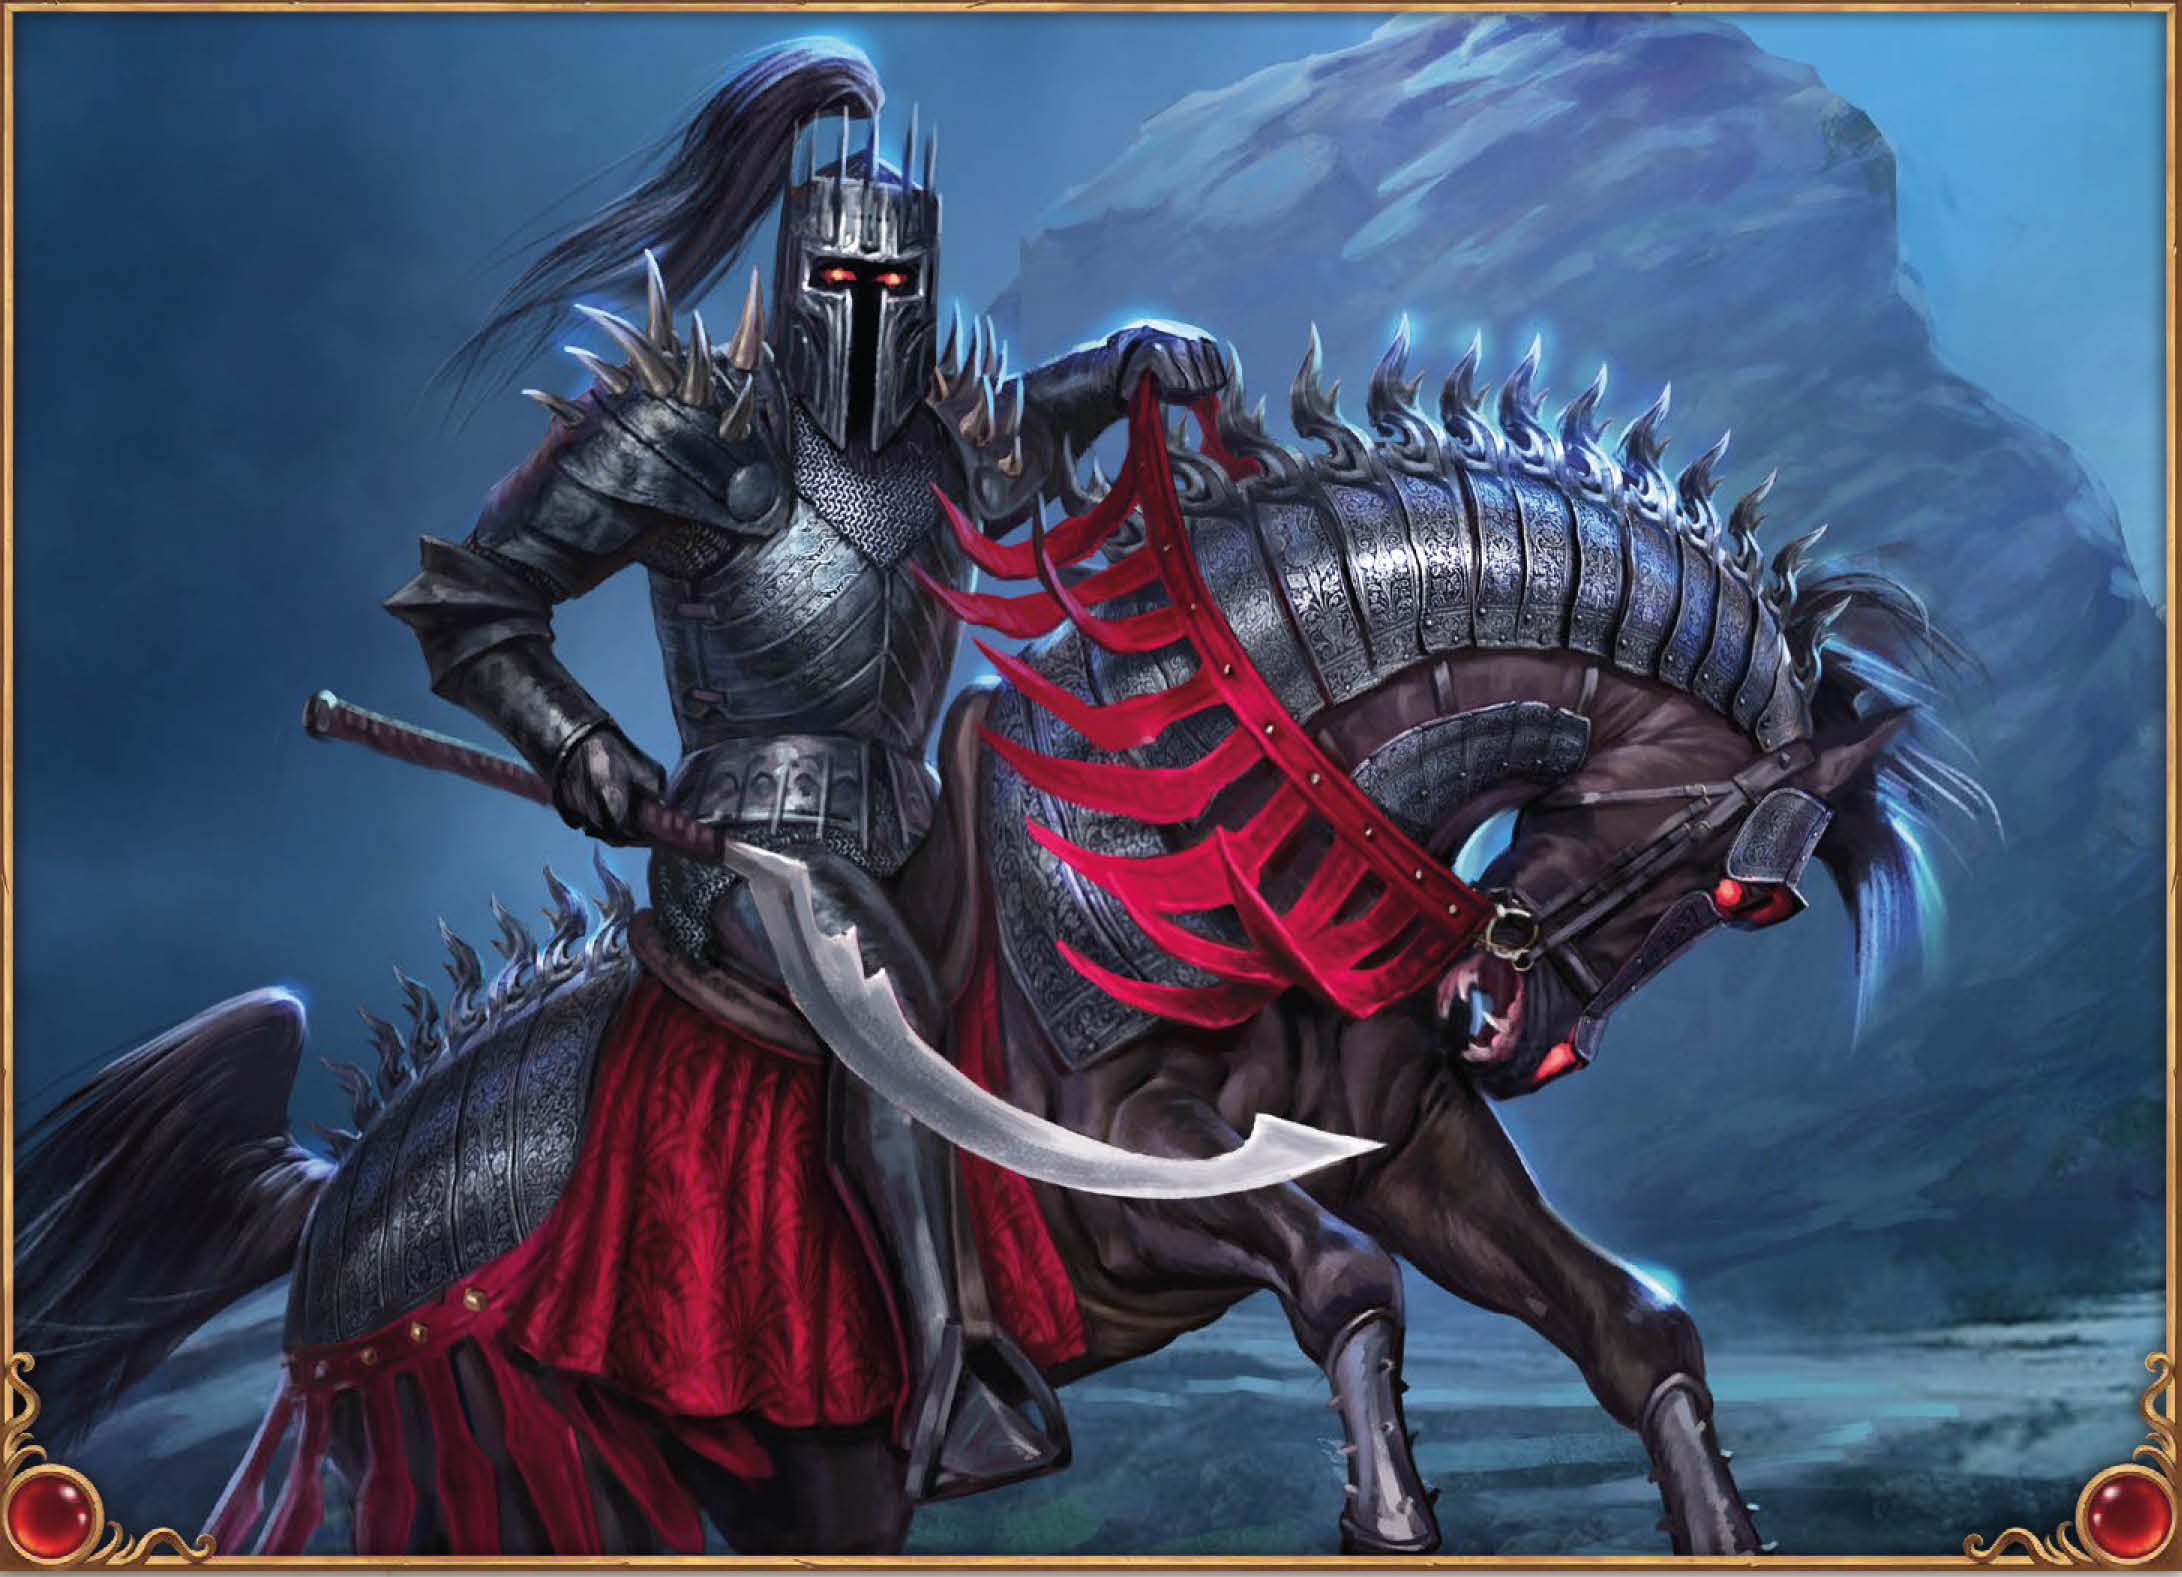
\includegraphics[width=\linewidth, height=\myspace, keepaspectratio]{\art/dread_knight.jpg}
\end{scaledfigure}

\clearpage

\subsection*{Combat Example}

\begin{multicols*}{2}
\textit{Bob's Zombies are about to attack Alice's Griffins.
As Bob announces the attack, both players now have a chance to modify the Attack or Defense of their own Unit by playing any number of \includesvg[height=10px]{\svgs/instant.svg} cards that increase an attacking Unit's \includesvg[height=10px]{\svgs/attack.svg} or a defending Unit's \includesvg[height=10px]{\svgs/defense.svg}.}\par
\textit{Bob decides to play a +1 Attack Card, increasing the Zombies' attack from 2 to 3.
Alice responds by playing a +1 Defense Card, increasing the Griffins' Defense from 0 to 1.
They would both be permitted to play any number of additional cards in any order, but they decide to stop after playing these cards.}\par

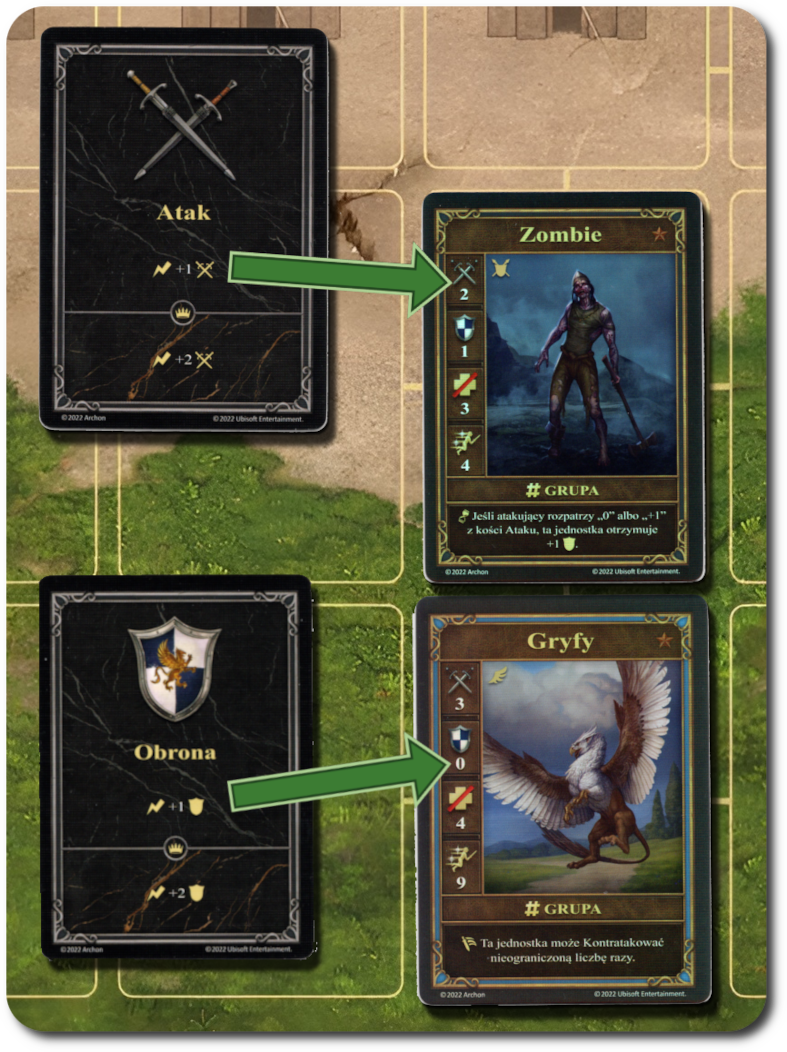
\includegraphics[width=\linewidth]{\examples/zombies_attack_griffins.png}

\textit{After all cards for the attack have been played, the Attack Die is thrown to further modify the amount of damage the attacking Unit deals.
Bob throws a +1.
This increases the Zombies' attack from 3 to 4, which is then reduced by the Griffins' Defense of 1. Therefore, 3 damage \includesvg[height=10px]{\svgs/damage.svg} is placed on the Griffins. Since they have a HP \includesvg[height=10px]{\svgs/health_points.svg} of 4, they are not flipped over to their "Few" side.}\par
\textit{The Griffins do not have a black cube on them, therefore they now start a Retaliation Attack.
The cube would now normally be placed on them, however their Special \includesvg[height=10px]{\svgs/unit_retaliate.svg} Ability indicates that they may Retaliate any number of times so the cube is not placed.}\par
\textit{Both players are allowed to modify the Statistics of their Units again during the Retaliation Attack.
The previously played Attack and Defense cards no longer have any effect.}

\vfill

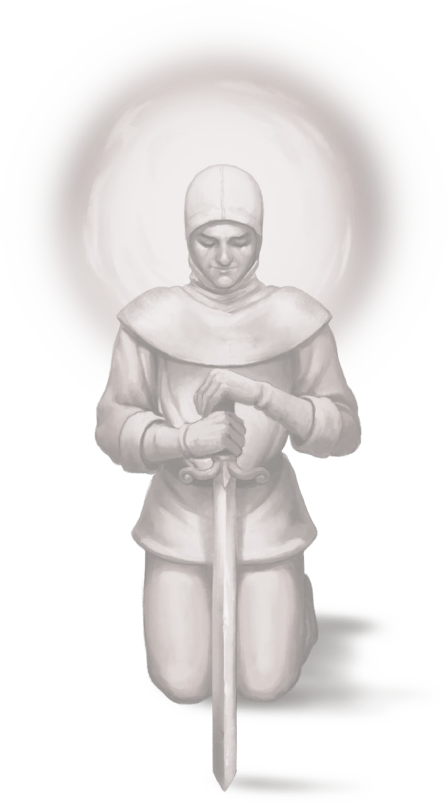
\includegraphics[width=\linewidth]{\art/prayer.png}

\end{multicols*}
